\section {System Overview\\}

\subsection{Design Goals and Rationale\\}
The design of the PushUp server is driven by the following rationales.
\begin{itemize}
\item {\bf Large Concurrent Connections}:
    As the long polling technologies requires the server to keep the polling
    request active for a period of time, large number of concurrent clients 
    will generate lots of active connections. One of the most goal of PushUp
    is to minimize the cost of maintaining these active concurrent connections,
    which can in turn enhance the system's scalability.
     
    The key to reduce the cost is the event-based notification mechanism 
    provided by the operating systems. Unlike the multi-process or 
    multithreading concurrent model, the event-based concurrency model 
    requires much less resource to maintain the connections.

\item {\bf Transparency}: Although event-based concurrency significantly 
    reduce the maintenance cost, it is impractical to have all the web 
    server to be implemented in event-based programming style. Thus, the 
    PushUp server provides the dedicated event-based long polling services
    for all underlying web servers. We hope the introduction of PushUp server
    requires minimal modification on the web servers and hides its existence
    from the clients.

\item {\bf Low Latency}: Adding an intermediate layer in between of the 
    clients and web servers will inevitably create some overhead. 
    The PushUp server should make sure that the extra costs should be within
    an ``acceptable" range.

\item {\bf Scalability}: The PushUp Server is designed to handle large number of
    active connections. We introduces mechanisms to make PushUp more able to
    handle this problem. 

\end{itemize}

\subsection{System Overview\\}

TODO: a figure to illustrate the main idea.

\begin{figure}[htb!]
\centering%
    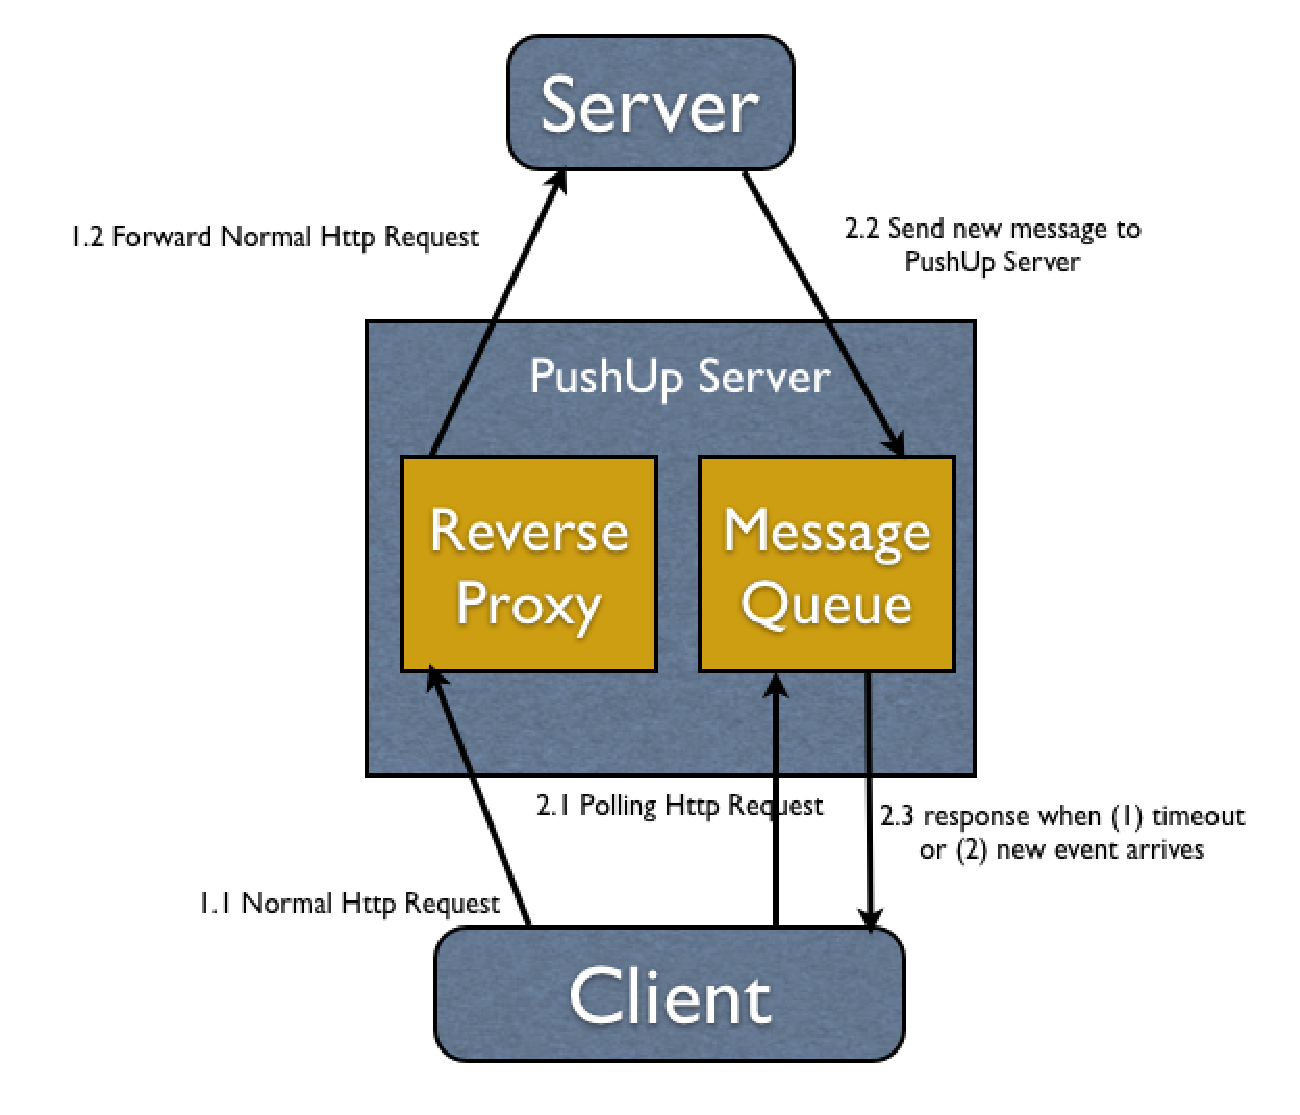
\includegraphics[scale=0.40]{figures/simple_pushup_arch.eps}
    \caption{Simplified PushUp Architecture}
    \label{fig:eventloop}
\end{figure}

TODO: Overall description of such design. and how it matches the rationale mentioned above.

TODO: should add add picture with the detailed architecture of the PushUp Server.

